\chapter{Tecnologie utilizzate}
\label{chap:2}

\section{Introduzione alle tecnologie}
\label{sec:IntroduzioneTecnologie}
Come già introdotto brevemente nel capitolo \ref{chap:1}, per lo scopo di questa tesi si è scelto di confrontare due approcci differenti, ma sempre più utilizzati nelle applicazioni web moderne.
In particolare si partirà da WebAssembly e dall'interfaccia di sistema WASI, per finire con un'introduzione anche su Node.js.

\section{WebAssembly}
\label{sec:Wasm}
WebAssembly (Wasm) è uno standard che definisce un formato binario (.wasm) e un relativo formato testuale (.wat) per la scrittura di codice eseguibile nelle pagine web. 
Wasm è attualmente sviluppato in maniera open-source, da un \emph{Community Group} del W3C che comprende membri di tutti i browser più utilizzati.
\\Esso è nato principalmente come integrazione a JavaScript, per consentire l'esecuzione di codice ad una velocità paragonabile a quella del codice nativo, grazie alla dimensione ridotta dei file binari generati e alla loro efficienza.
\\Inoltre grazie all'esecuzione all'interno di una sandbox è garantita un ottima sicurezza, anche sotto il punto di vista della memoria.
\\Grazie al formato testuale (.wat), è possbile eseguire debug, test, ottimizzazioni, scrivere a mano programmi di basso livello, ma anche visualizzare i sorgenti dei moduli wasm, quando questi sono utilizzati una pagina web.
\cite*{wasmDesign}
\\Al giorno d'oggi è in costante crescita, sia il numero di linguaggi che possono avere come \emph{compilation target} WebAssembly (Rust, C, Go, Kotiln, etc), sia il numero di siti che sfruttano tale tecnologia, grazie anche al fatto che praticamente ogni browser attualmente utilizzato, supporta Wasm. 
\begin{figure}
        \begin{center}
                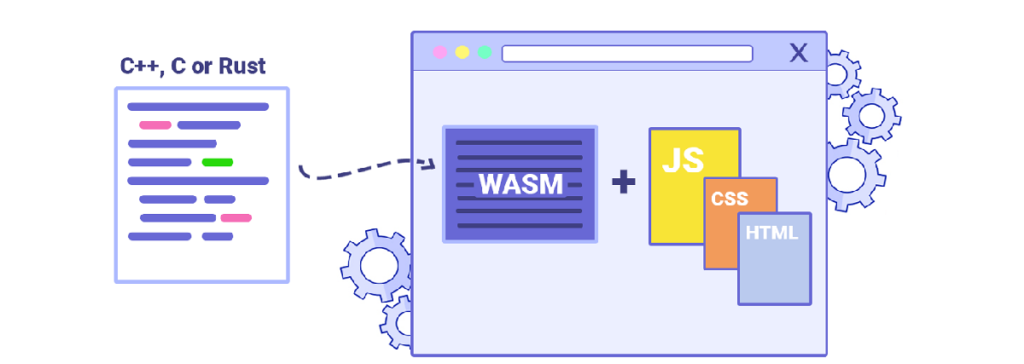
\includegraphics[width=0.8\columnwidth]{images/wasm.png}
        \end{center}
        \caption{WebAssembly all'interno del browser}
        \label{fig:wasm}
\end{figure}
\subsection{Storia e Origini}
\subsubsection{I predecessori}
Nel 2011 Google rilasciò un progetto open source chiamato \textbf{Native Client (NaCl)}.
L'obiettivo era quello di consentire l'esecuzione di codice nativo nel browser all'interno di una sandbox con privilegi limitati.
In particolare si stava cercando di supportare software che richiedevano grande sforzo computazionale (simulazioni, elaborazioni di audio e video e giochi).
\\Il progetto si rivelò un successo sotto il punto di vista prestazionale. Vennero infatti rilasciati diversi software e giochi che presentavano prestazioni simili alla rispettiva versione Desktop.
Non mancavano però diversi problemi. Il codice ottenuto era eseguibile solo nel browser Chrome ed era impossibile l'interazione con JavaScript o con altre API sul web.
\\Un tentativo di evoluzione fu presentato nel 2013 dal team di Mozilla. Si trattava di \textbf{asm.js}, un sottoinsieme di JavaScript che consentiva l'invocazione di funzioni scritte in linguaggi come C, C++ o Rust, in diversi browser e direttamente da JavaScript.
A discapito di una maggior portabilità ci fu una significativa diminuizione delle prestazioni, dovuta alla lentezza dell'interprete JavaScript, che era stato caricato di un notevole overhead.
\\Queste due soluzioni dimostrarono la possbilità di eseguire codice in una sandbox, o con ottime prestazioni, ma solo all'interno di Chrome (NaCl), oppure in diversi browser ma con prestazioni decisamente inferiori.
Si voleva quindi trovare un modo per unificare gli enormi vantaggi offerti da ognuno dei due approcci.\cite*{wasmBook}
\subsubsection{La nascita di Wasm}
Fu nel Giugno 2015 che Brendan Eich (creatore di JavaScript), insieme ad altri sviluppatori di Mozilla, annunciarono che lo sviluppo di WebAssembly era cominciato.\cite*{asmjsToWasm}
Wasm venne presentato come "un nuovo standard open source che definiva un formato e un modello di esecuzione portabile, efficiente in termini di dimensioni e tempo di caricamento, specificamente progettato per essere un target di compilazione per il web".
WebAssembly prometteva prestazioni fino a 20 volte superiori rispetto ad asm.js, grazie alla maggiore velocità di decodifica dei file binari rispetto a quella di parsing da parte dell'interprete JavaScript per i file di asm.js.
Nel 2017 venne lanciato il \emph{minimum viable product} (MVP), che conteneva pressochè le stesse funzionalità presenti in asm.js e venne dichiarata conclusa la fase di preview.
Capendo le potenzialità di ciò che stava venendo sviluppato hanno dato il loro contributo al progetto, aziende del calibro di Google, Microsoft, Apple, Unity.

\subsection{Casi d'uso}
Inizialmente ci si è concentrati sull'utilizzo di WebAssembly all'interno del browser e venivano presentati svariati casi d'uso:
\begin{itemize}
        \item Elaborazione di immagini e video
        \item Giochi
        \item Applicazioni peer-to-peer
        \item Applicazioni CAD
        \item Realtà virtuale e realtà aumentata con latenza minima
        \item Riconoscimento di immagini
        \item Simulazione/emulazioni di sistemi operativi (QEMU, DOSBox)
        \item Applicazioni per desktop ridimensionamento
        \item Web server locali
\end{itemize}
Si era pensato fin da subito anche alla portabilità ed erano stati presentati diversi possibili utilizzi anche per ambienti non-web:
\begin{itemize}
        \item Esecuzione server-side di codice non attendibile
        \item Servizi per la distribuzione di giochi
        \item Generiche applicazioni server side
        \item Calcolo simmetrico, distribuito su più nodi
\end{itemize}
\subsection{Concetti chiave}
WebAssembly codifica un linguaggio di programmazione di basso livello, simile ad Assembly. Tale linguaggio è strutturato attorno ai seguenti concetti:\cite*{wasmSpec}

\subsubsection{Valori}
In WebAssembly sono presenti:
\begin{itemize}
        \item Un tipo \emph{byte} per la rappresentazione di byte non interpretati
        \item Quattro tipi di valori numerici: interi e numeri a virgola mobile, ognuno da 32 o 64 bit (\emph{i32, i64, f32, f64})
        \item Un tipo vector a 128 bit(\emph{i128}) contenente anch'esso valori numerici (ad esempio da 2 f64, oppure da 4 i32 etc.)
        \item Un tipo riferimento per puntatori a differenti entità.
\end{itemize}
Quest'ultimo è definito "opaco", in quanto non è visibile né la loro dimensione, né la loro rappresentazione in bit. Al contrario i primi due tipi si dicono "trasparenti".
\\Infine è anche possibile .
\subsubsection{Istruzioni}
Il modello computazionale di WebAssembly è basato su uno stack. Il codice è costituito da una sequenza di istruzioni eseguite in ordine. Le istruzioni sfruttano una struttura dati detta \emph{operand stack} e possono essere di tipo semplice, o di controllo.
\\Le operazioni semplici svolgono manipolazioni basilari sui dati, prelevando parametri dallo stack (\emph{pop}) e inserendo il risultato nello stesso (\emph{push}). Le operazioni di controllo, si occupano invece di alterare il flusso di esecuzione grazie a costrutti condizionali, blocchi e cicli.
\subsubsection{Traps} 
Alcune istruzioni possono fallire e generare degli errori (traps) che non è possibile gestire all'interno di WebAssembly. Tali errori vengono infatti lanciati nell'ambiente di esecuzione dell'host dove, al contrario, vengono normalmente gestiti.
\subsubsection{Funzioni}
Il codice è diviso in funzioni. Ognuna di queste ha una certe sequenza di valori sia come parametri che come tipo di ritorno. In una funzione viene eseguita una serie di istruzioni, possono inoltre essere chiamate altre funzioni (anche ricorsivamente) e create variabili locali.
\subsubsection{Tabelle}
Una tabella è un array di valori "opachi" di un particolare tipo. Tale struttura consente al programma di ottenere i valori indirettamente attraverso un indice dinamico. Tramite le tabelle è possibile, per esempio invocare funzioni indirettamente, emulando in questo modo i puntatori a funzione.
\subsubsection{Memoria lineare}
La memoria lineare è un  array continuo di byte. Ha una dimensione iniziale che può crescere dinamicamente al bisogno. Un programma può leggere e scrivere valore in memoria (operazioni di \emph{load/store}) in un qualsiasi indirizzo al suo interno (anche in maniera non allineata).
\subsubsection{Moduli}
Un modulo è l'unità di deployment per un programma WebAssembly. Esso conterrà le definizioni di funzioni, tabelle, memoria etc. In un modulo è anche possibile esportare o importare definizioni, inizializzare tabelle o memoria lineare e anche definire una funzione \emph{start} che verrà eseguita automaticamente. 
\subsubsection{Embedder}
Solitamente un modulo WebAssembly sarà integrato in un host che ne definirà l'inizializzazione, la risoluzione delle funzioni importate  e le modalità di accesso di quelle esportate. L'Embedder è l'entità che implementa la connessione tra l'ambiente host e il modulo Wasm. Ci si aspetta che l'embedder interagisca con la semantica di WebAssembly in un modo ben definito nelle specifiche del formato Wasm.
\begin{figure}
        \begin{center}
                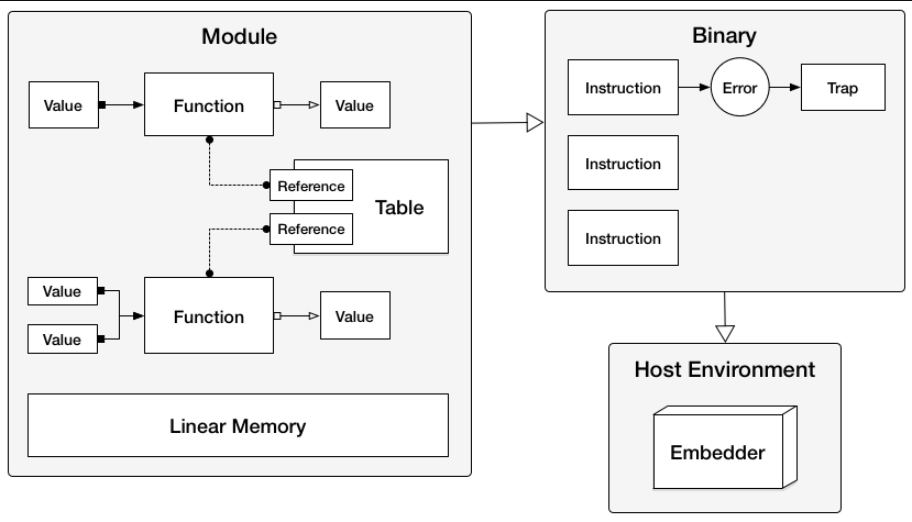
\includegraphics[width=0.9\columnwidth]{images/wasmArchitecture.png}
        \end{center}
        \caption{Architettura di WebAssembly}
        \label{fig:wasmArch}
\end{figure}
\newpage
\subsection{Fasi semantiche}
Nella semantica di WebAssembly è possibile individuare tre fasi principali: decodifica, validazione ed esecuzione.\cite*{wasmSpec}
\subsubsection{Decodifica}
I moduli WebAssembly sono distribuiti in formato binario (.wasm) e per questo è necessario decodificarli in modo da ottenere una rappresentazione interna del modulo, con cui il web browser o il runtime environment potrà lavorare.
\subsubsection{Validazione}
Dopo aver decodificato i moduli binari, per poterli istanziare, è necessario controllare che questi siano validi.
La validità è verificata grazie ad un sistema di tipi basato sulla sintassi astratta di un modulo e sul suo contenuto. In particolare per ogni componente della sintassi è presente una regola che specifica le condizioni da rispettare perchè il modulo risulti valido.
\begin{figure}
        \begin{center}
                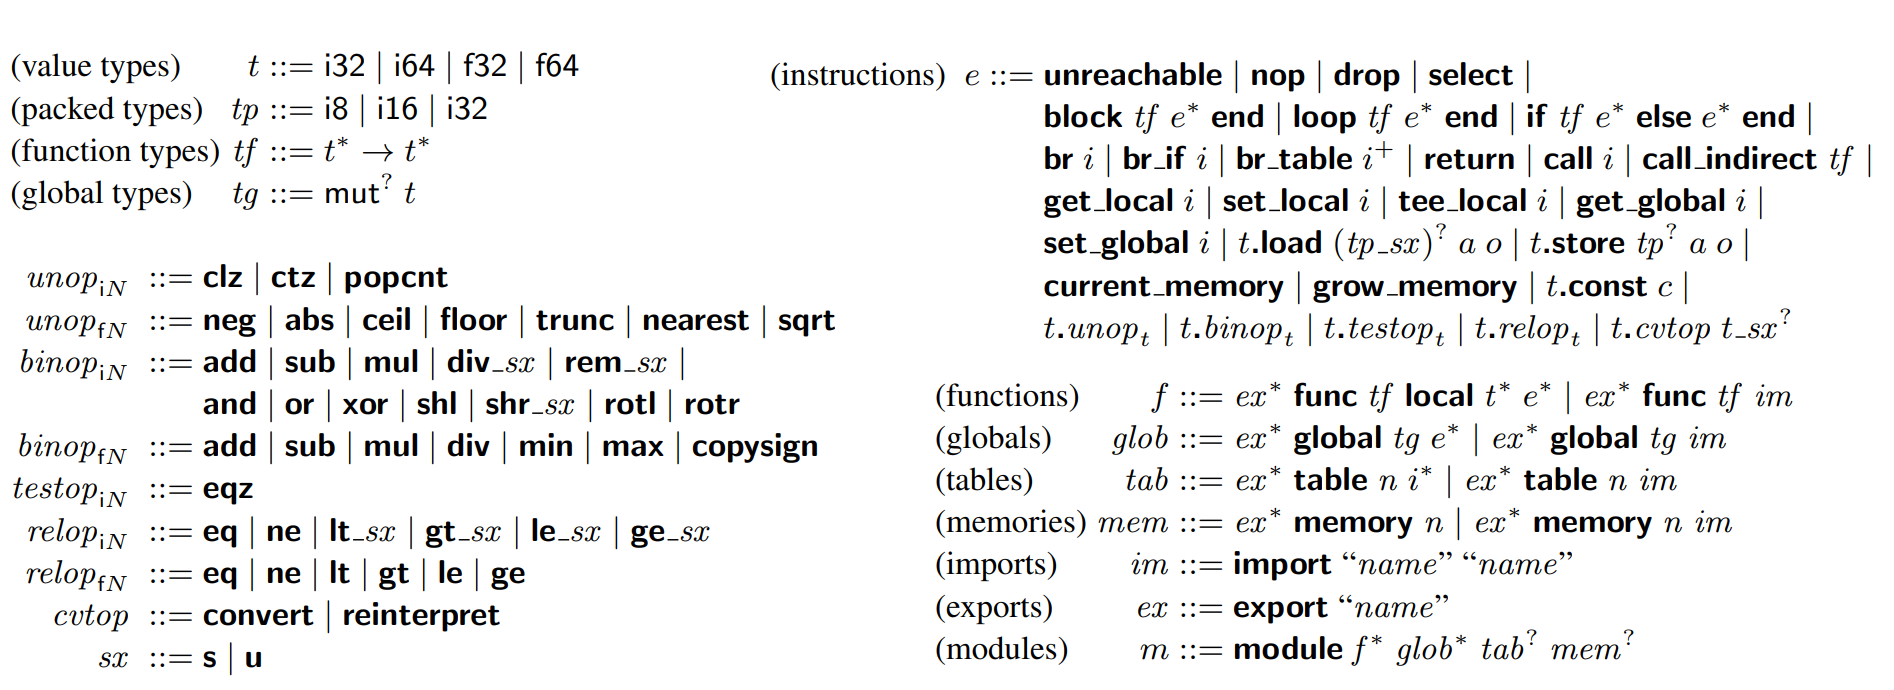
\includegraphics[width=1\columnwidth]{images/wasmSyntax.png}
        \end{center}
        \caption{La sintassi astratta di WebAssembly}
        \label{fig:wasmSyntax}
\end{figure}
\\Ad esempio viene controllato l'ordine delle istruzioni nel corpo di una funzione assicurandosi che lo stack sia utilizzato nel modo corretto.
Oppure se nelle specifiche esaminiamo un'operazione binaria tra tipi numerici (i32.add, f64.xor etc.), notiamo che essa è del tipo \emph{t.binop} e dato un contesto \(C\) essa è valida solamente con tipo \([t~t]{\rightarrow} [t]\).
\\Tale regola si può anche rappresentare con la seguente notazione formale:
\begin{equation*}
\frac{
}{
        C {\vdash} t\mathsf{.}{\mathit{binop}} : [t~t] {\rightarrow} [t]
}
\end{equation*}
Esaminando invece le regole di validazione di un'istruzione per l'aumento di memoria lineare \emph{memory.grow} (tale istruzione si aspetta l'offset che indica di quanto la memoria è da espandere e ritorna la dimensione della memoria precedente all'espansione) notiamo che:
\begin{itemize}
        \item La memoria \(C.{\mathit{mems}}[0]\) deve essere definita nel contesto.
        \item Allora l'istruzione risulta valida con tipo \([{\mathit{i32}}] {\rightarrow} [{\mathit{i32}}]\)
\end{itemize}
In notazione formale:
\begin{equation*}
        \frac{
        C.{\mathit{mems}}[0] = {\mathit{memtype}}
      }{
        C {\vdash} {\mathit{memory.grow}} : [{\mathit{i32}}] {\rightarrow} [{\mathit{i32}}]
      }        
\end{equation*}
\subsubsection{Esecuzione}
Terminata la validazione di ogni istruzione il modulo può finalmente essere istanziato.
L'istanza di un modulo ne è la rappresentazione dinamica. Esso comprende lo stack, sul quale operano le istruzioni WebAssembly e uno \emph{\textbf{store}} astratto, contenente lo stato globale (è la rappresentazione a runtime di tutte le istanze di funzioni, tabelle, memorie etc. che sono state allocate dall'istanziazione).
Terminata l'istanziazione, diventa effettivamente possibile l'esecuzione di istruzioni WebAssembly.
\\In particolare, se nel modulo era stata definita una funzione \emph{\_start}, essa sarà eseguita subito dopo la creazione dell'istanza, altrimenti sarà possibile invocare funzioni esportate, chiamandole direttamente dall'istanza stessa.
\\Per ogni istruzione, è presente una regola che specifica l'effetto della sua esecuzione sullo stato del programma. Rimanendo coerenti con gli esempi sulla validazione, segue il comportamento dell'istruzione \emph{t.binop}:

\begin{itemize}
        \item In seguito alla validazione, possiamo assumere che due valori di tipo \(t\) si trovino in cima allo stack.
        \item Viene eseguita l'operazione di \textbf{pop} del valore \(t.const~c_1\) dallo stack
        \item Viene eseguita l'operazione di \textbf{pop} del valore \(t.const~c_2\) dallo stack
        \item Se \({\mathit{binop}}_t(c_1, c_2)\) è definita allora:
        \begin{itemize}
                \item Sia \(c\) il possibile risultato di \({\mathit{binop}}_t(c_1, c_2)\)
                \item Viene eseguita l'operazione di \textbf{push} del valore \(t.const~c\) nello stack
        \end{itemize}
        \item Altrimenti:
        \begin{itemize}
                \item Trap
        \end{itemize}
\end{itemize}
In notazione formale:
\begin{equation*}
        \begin{split}\begin{array}{lcl@{\qquad}l}
                (t\mathsf{.}{\mathsf{const}}~c_1)~(t\mathsf{.}{\mathsf{const}}~c_2)~t\mathsf{.}{\mathit{binop}} &{\hookrightarrow}& (t\mathsf{.}{\mathsf{const}}~c)
                  & (\mathrel{\mbox{if}} c \in {\mathit{binop}}_t(c_1,c_2)) \\
                (t\mathsf{.}{\mathsf{const}}~c_1)~(t\mathsf{.}{\mathsf{const}}~c_2)~t\mathsf{.}{\mathit{binop}} &{\hookrightarrow}& {\mathsf{trap}}
                  & (\mathrel{\mbox{if}} {\mathit{binop}}_{t}(c_1,c_2) = \{\})
                \end{array}\end{split}
\end{equation*}
Non viene riportato l'esempio anche sull'istruzione \emph{memory.grow} essendo una funzionalità decisamente più complessa (11 diversi passaggi, con svariati sottocasi) che comporterebbe obbligatoriamente, l'introduzione di ulteriori dettagli che esulano dallo scopo di questa tesi.
\break
Si noti che sia l'istanziazione, che l'invocazione di funzioni, sono operazioni che avvengono all'interno dell'ambiente di esecuzione dell'host.
\begin{figure}
        \begin{center}
                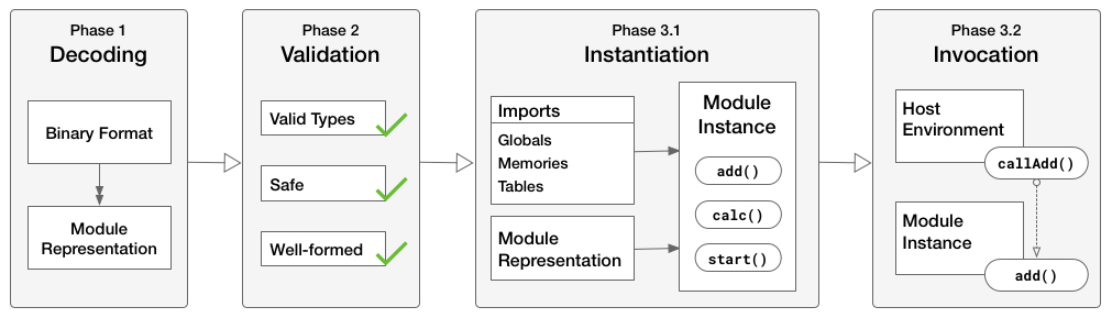
\includegraphics[width=0.97\columnwidth]{images/wasmSemanticPhases.png}
        \end{center}
        \caption{La semantica di WebAssembly}
        \label{fig:wasmPhases}
\end{figure}

\newpage
\subsection{Correttezza logica}
Grazie alla sua semantica è possibile dire che il sistema di tipi di WebAssembly è logicamente corretto (\emph{sound})\cite*{wasm:soundness}. Esso infatti garantisce sia \emph{\textbf{type safety}}, che \emph{\textbf{memory safety}}.
\\Per quanto riguarda la sicurezza rispetto ai tipi, tutti i tipi controllati durante la validazione saranno rispettati anche a runtime:
\begin{itemize}
        \item Ogni variabile (locale o globale) conterrà valori del tipo corretto
        \item Ogni istruzione verrà applicata solo ad operandi del tipo che ci si aspetta e restituirà valori del tipo corretto
        \item Ogni funzione restituirà valori del tipo previsto, a meno di errori (trap)
\end{itemize}
Per quanto riguarda la \emph{memory safety}, è garantito che non verrà acceduta nesun'area di memoria, diversa da quelle esplicitamente specificate dal programma. Ogni volta che per esempio verrà fatta un'operazione di load/store in un certo indirizzo di memoria, si controllerà che quest'ultimo sia nel range di indirizzi possibili per l'istanza attuale di WebAssembly.
\\Inoltre sono garantite altre proprietà: 
\begin{itemize}
        \item L'assenza di comportamenti indefiniti: le regole di esecuzione sono mutualmente consistenti e coprono qualsiasi caso che possa capitare in un programma validato
        \item L'incapsulamento per funzioni e moduli: nessuna variabile locale può essere acceduta fuori dalla funzione dove è dichiarata e nessun componente di un modulo può essere acceduto fuori dallo stesso a meno che quest'ultimo non sia esportato o importato
\end{itemize}
Infine è importante notare che le regole di validazione si occupano solamente dei componenti statici di un programma WebAssembly. Per dimostrare correttezza in maniera precisa, sono state estese le \emph{typing rules} anche ai componenti dinamici, come lo \textbf{store}, le \textbf{configurations} (coppie Store - Thread di esecuzione) e le istruzioni amministrative.
Dopo aver dato la definizioni di configurazione valida è stato possibile enunciare due teoremi e derivare un corollario che riassumendo dicono che:
\\Ogni thread in una \emph{configuration} valida o esegue per sempre, o termina con un errore (trap), o termina con un risultato del tipo atteso. Di conseguenza, dato uno \emph{store} valido, nessun calcolo derivante dall'istanzazione o dall'invocazione di un modulo valido, può avere comportamenti diversi da quelli definiti nelle specifiche. \cite*{wasm:soundness:theorems}
\subsection{Creazione e utilizzo di moduli WebAssembly}
Sebbene sia possibile scrivere a mano il codice dei moduli WebAssembly, è molto più comune scrivere il codice in un linguaggio di alto livello e poi compilare quest'ultimo in un modulo Wasm.
Nonostante durante lo sviluppo iniziale del linguaggio ci si fosse concentrati solo sull'utilizzo di C/C++, ad oggi sono più di 10 i linguaggi che supportano WebAssembly come \emph{compilation target}. Tra questi spiccano Rust, C\#, Python, Kotlin, Swift, Go. 
\\Per esempio, utilizzando Rust sarebbe sufficiente scrivere un normale programma e poi lanciare il seguente comando nella directory del progetto: 
\begin{lstlisting}[language=Bash, numbers=none, label=lst:RustCompile, caption={}]
wasm-pack build
\end{lstlisting}
Tale comando compilerà il programma in un modulo WebAssembly, generando un file \textbf{.wasm} utilizzabile dal codice JavaScript della nostra pagina web.
\\Bisogna però sottolineare che sin dagli albori di WebAssembly, non era mai stata fatta nessuna assunzione sull'ambiente host e che il utilizzo non sarebbe stato limitato alle sole pagine web.
\\In particolare, per lo scopo di questa tesi, sarà necessario che i moduli WebAssembly vengano istanziati ed eseguiti server side, ma soprattuto che tali moduli abbiano accesso al \textbf{file system} e a funzioni di \textbf{I/O}.
Tali funzioni in WebAssembly non sono disponibili, a causa dell'esecuzione all'interno di una sandbox e delle caratteristiche di sicurezza. Per questi e per molti altri motivi è stato sviluppato WASI (WebAssembly System Interface).
\newpage
\section{WebAssembly System Interface}
\label{sec:WASI}
\subsection{Ruolo di WebAssembly System Interface}
\subsection{Rust e WASI}
\subsection{Struttura di WASI}
\subsection{Wasmtime}
\subsection{Applicazioni e Casistiche d'Uso di WASI}

\newpage
\section{Node.js}
\label{sec:Node}
\subsection{Panoramica di Node.js}
\subsection{Vantaggi di Node.js}
\subsection{Ecosistema di Node.js}

\newpage
\section{Confronto tra tecnologie}
\label{sec:Confronto}
\subsection{Prestazioni}
\subsection{Sicurezza}
\subsection{Facilità di Sviluppo}
\subsection{Scalabilità ed Espandibilità}

\newpage
\section{Conclusioni preliminari}
\label{sec:ConclusioniTecnologie}

\newpage
\lstinputlisting[label=lst:hello, firstline=2, lastline=4, caption={I directly included a portion of a file}]{code/hello.py}

\begin{lstlisting}[language=Java, label=lst:java, caption={Some code in another language than the default one}]
public void prepare(AClass foo) {
        AnotherClass bar = new AnotherClass(foo)
}
\end{lstlisting}
